\documentclass[11pt]{article}

\usepackage[margin=1in]{geometry}
\usepackage{amsmath,amssymb}
\usepackage{tikz}
\usetikzlibrary{positioning, arrows.meta, shapes.geometric, fit, calc, backgrounds, decorations.pathreplacing}
\usepackage{graphicx}
\usepackage{hyperref}
\usepackage{booktabs}
\usepackage{caption}
\usepackage{subcaption}
\usepackage{float}
\usepackage{enumitem}
\usepackage{xcolor}

% Brand colors
\definecolor{Garnet}{HTML}{73000A}
\definecolor{Atlantic}{HTML}{466A9F}
\definecolor{Congaree}{HTML}{1F414D}
\definecolor{Rose}{HTML}{CC2E40}
\definecolor{Horseshoe}{HTML}{65780B}
\definecolor{Grass}{HTML}{CED318}
\definecolor{Honeycomb}{HTML}{A49137}
\definecolor{LightGray}{HTML}{ECECEC}
\definecolor{Black90}{HTML}{363636}
\definecolor{Black70}{HTML}{5C5C5C}
\definecolor{Black50}{HTML}{A2A2A2}
\definecolor{Sandstorm}{HTML}{FFF2E3}

\hypersetup{colorlinks=true, linkcolor=Garnet, urlcolor=Atlantic, citecolor=Congaree}

\title{
\textbf{Plug-and-Play Prompt Optimization} \\[0.3em]
\Large One-Shot Segmentation via Q-Learning on \\
Dual-Space Heterogeneous Graphs \\[0.5em]
\normalsize A Technical Explainer of the PPO Pipeline (Liu et al., CVPR 2025)
}

\author{J.C. Vaught}
\date{February 2026}

\begin{document}
\maketitle

\begin{abstract}
This document provides a detailed technical walkthrough of the Plug-and-Play Prompt Optimization (PPO) pipeline for one-shot image segmentation. The system combines DINOv2 feature matching, a dual-space heterogeneous graph representation, tabular Q-learning with experience replay, and the Segment Anything Model (SAM) to segment objects in unseen images given only a single reference example. We explain every component with mathematical formulations, architectural diagrams, and experimental results from a real underwater segmentation task (blue tang fish on coral reef), where the pipeline improved SAM mask IoU from 0.001 to 0.760 after 30 training episodes.
\end{abstract}


\newpage

% ============================================================
\section{Problem Statement}
% ============================================================

The Segment Anything Model (SAM) produces high-quality segmentation masks but requires user-provided \textit{prompts}: point coordinates labeled as positive (``segment here'') or negative (``not here''). The quality of SAM's output is extremely sensitive to prompt placement. Moving a single point by a few pixels can change the mask from a tight object boundary to a background region covering 87\% of the image.

The goal of \textit{one-shot segmentation} is to segment an object in a new \textit{target} image given only a single \textit{reference} image with a ground-truth mask. The challenge is automatically generating effective SAM prompts for the target image without any manual intervention or model retraining.

Figure~\ref{fig:sensitivity} demonstrates the prompt sensitivity problem on a real underwater image. In the first panel, prompts placed on the coral cause SAM to select the wrong object entirely, segmenting the background instead of the fish. The second panel shows the optimal case: a single well-placed positive prompt produces a near-perfect mask of the blue tang. The third panel illustrates that over-prompting can be counterproductive --- too many positive and negative points cause SAM to lock onto the wrong regions, such as the black markings on the fish rather than the full body.

\begin{figure}[H]
\centering
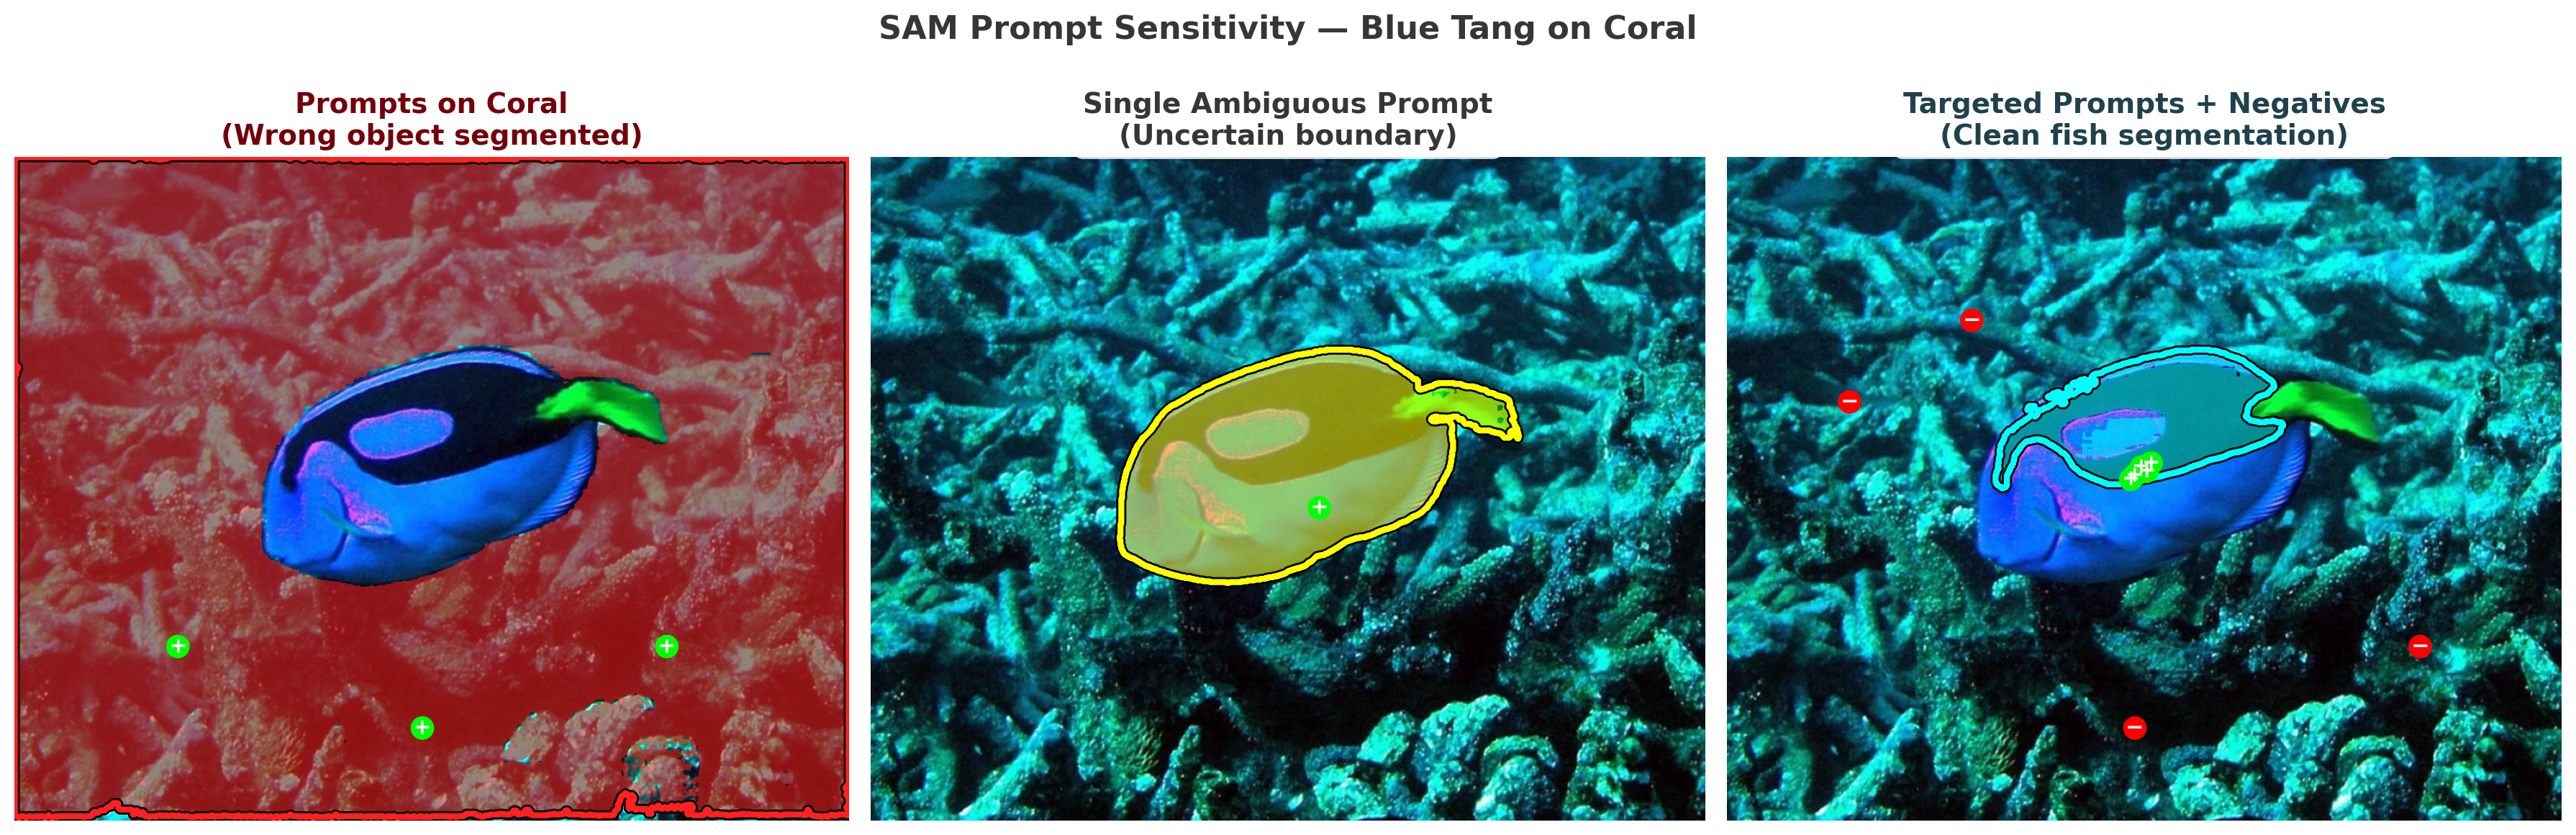
\includegraphics[width=\textwidth, trim=0 0 0 80pt, clip]{figures/bluetang_fig1_prompt_sensitivity.png}
\caption{SAM prompt sensitivity on the blue tang image.}
\label{fig:sensitivity}
\end{figure}

% ============================================================
\section{Pipeline Overview}
% ============================================================

The PPO pipeline has three stages executed sequentially. Figure~\ref{fig:problem} shows the full pipeline architecture. A single labeled reference example feeds into frozen DINOv2 ViT-G/14, which extracts 1536-dim patch features for both reference and target images. These features construct a dual-space heterogeneous graph (${\sim}$2M edges, 5 types), on which a tabular Q-learning agent optimizes prompt selection via graph-statistic rewards without ever calling SAM. The final Q-table is decoded into $(x,y)$ point prompts fed to frozen SAM ViT-B, which segments the target image in a single forward pass.

\begin{figure}[H]
\centering
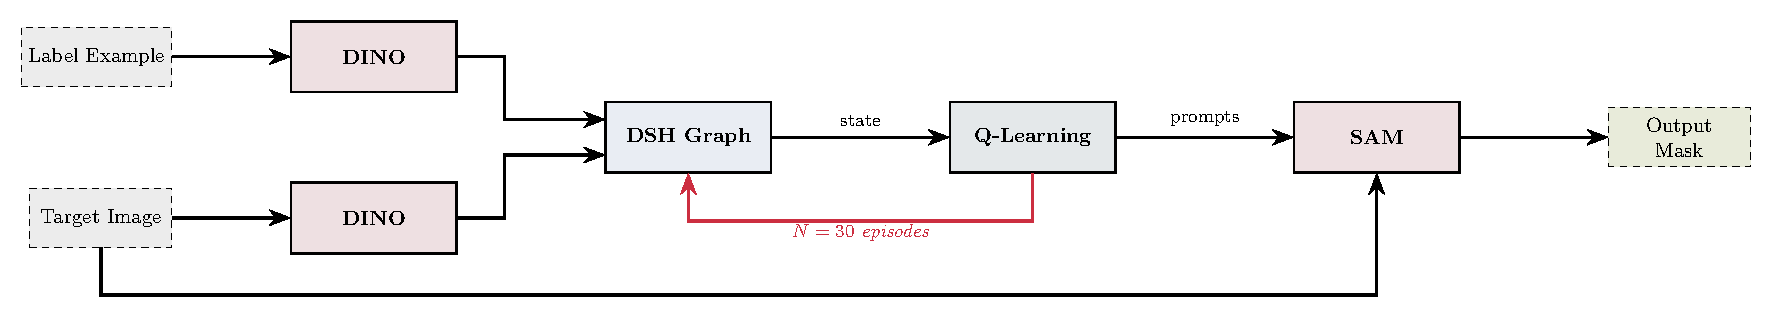
\includegraphics[width=\textwidth]{figures/fig_pipeline_highlevel.pdf}
\caption{Full PPO pipeline architecture.}
\label{fig:problem}
\end{figure}

The remaining figures in this document detail each stage individually. Figure~\ref{fig:dino_detail} shows how DINOv2 extracts and matches patch-level features between the reference and target images. Figure~\ref{fig:dsh_internals} illustrates the dual-space heterogeneous graph structure with its five edge types spanning feature space and physical space. Figure~\ref{fig:graph_detail} traces the graph construction and Q-learning optimization process using real pipeline outputs. Figure~\ref{fig:qlearning_mdp} diagrams the Q-learning MDP loop that drives prompt selection.

% ============================================================
\section{Step 1: DINOv2 Feature Matching}
% ============================================================

\subsection{Image Patchification}

Both the reference and target images are resized to $560 \times 560$ pixels. DINOv2 uses a Vision Transformer with \textbf{patch size 14}, dividing each image into a $40 \times 40 = 1{,}600$ grid of non-overlapping patches. Each patch occupies a $14 \times 14$ pixel region and receives a one-dimensional index computed as
\begin{align}
\texttt{index} = \texttt{row} \times 40 + \texttt{col}, \quad \text{where} \quad \texttt{row} = \lfloor y / 14 \rfloor, \quad \texttt{col} = \lfloor x / 14 \rfloor.
\end{align}
The center pixel of patch $i$ is at coordinates
\begin{align}
(c_x, c_y) = \left( (\texttt{col}_i \times 14) + 7, \; (\texttt{row}_i \times 14) + 7 \right).
\end{align}

\begin{figure}[H]
\centering
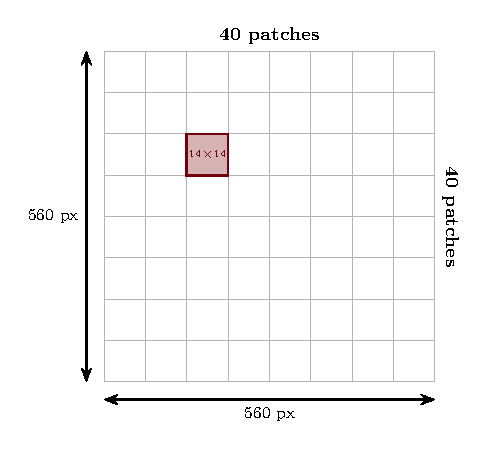
\includegraphics[width=0.5\textwidth]{figures/fig_patchification.pdf}
\caption{Patchification of the $560 \times 560$ input image into a $40 \times 40$ grid.}
\label{fig:patches}
\end{figure}

Figure~\ref{fig:patches} illustrates this grid. Each of the $40 \times 40 = 1{,}600$ patches occupies $14 \times 14$ pixels and is assigned a 1D index used throughout the pipeline.

\subsection{Foreground and Background Classification}

The reference image's ground-truth mask is scanned in $14 \times 14$ blocks. A block is classified as \textbf{foreground} if every pixel in that block is non-black (RGB $\neq [0,0,0]$), and as \textbf{background} if every pixel is black. Blocks with mixed content (partially on the object boundary) are discarded entirely. This produces two index sets: $\mathcal{F} = \{f_1, f_2, \ldots, f_{N_f}\}$ (foreground) and $\mathcal{B} = \{b_1, b_2, \ldots, b_{N_b}\}$ (background).

\subsection{DINOv2 Feature Extraction}

Both images are preprocessed with ImageNet normalization and passed through \textbf{DINOv2 ViT-G/14} ($\sim$1.1B parameters, $\sim$4.2 GB checkpoint). The model outputs patch-level features from the \texttt{x\_norm\_patchtokens} layer, yielding a tensor of shape $[2, 1600, 1536]$. For each of the 2 images, each of the 1600 patches receives a 1536-dimensional feature vector.
\begin{align}
\mathbf{F}^{\text{ref}} &= \text{DINOv2}(I_{\text{ref}}) \in \mathbb{R}^{1600 \times 1536} \\
\mathbf{F}^{\text{tgt}} &= \text{DINOv2}(I_{\text{tgt}}) \in \mathbb{R}^{1600 \times 1536}
\end{align}

Figure~\ref{fig:dino_detail} shows this process in detail. The reference image with its ground-truth mask and the target image are both passed through frozen DINOv2 ViT-G/14. PCA visualization of the 1536-dim patch features reveals that the model separates the fish from the coral background in feature space. Cosine similarity matching between reference foreground patches and all target patches produces initial positive prompt candidates.

\begin{figure}[H]
\centering
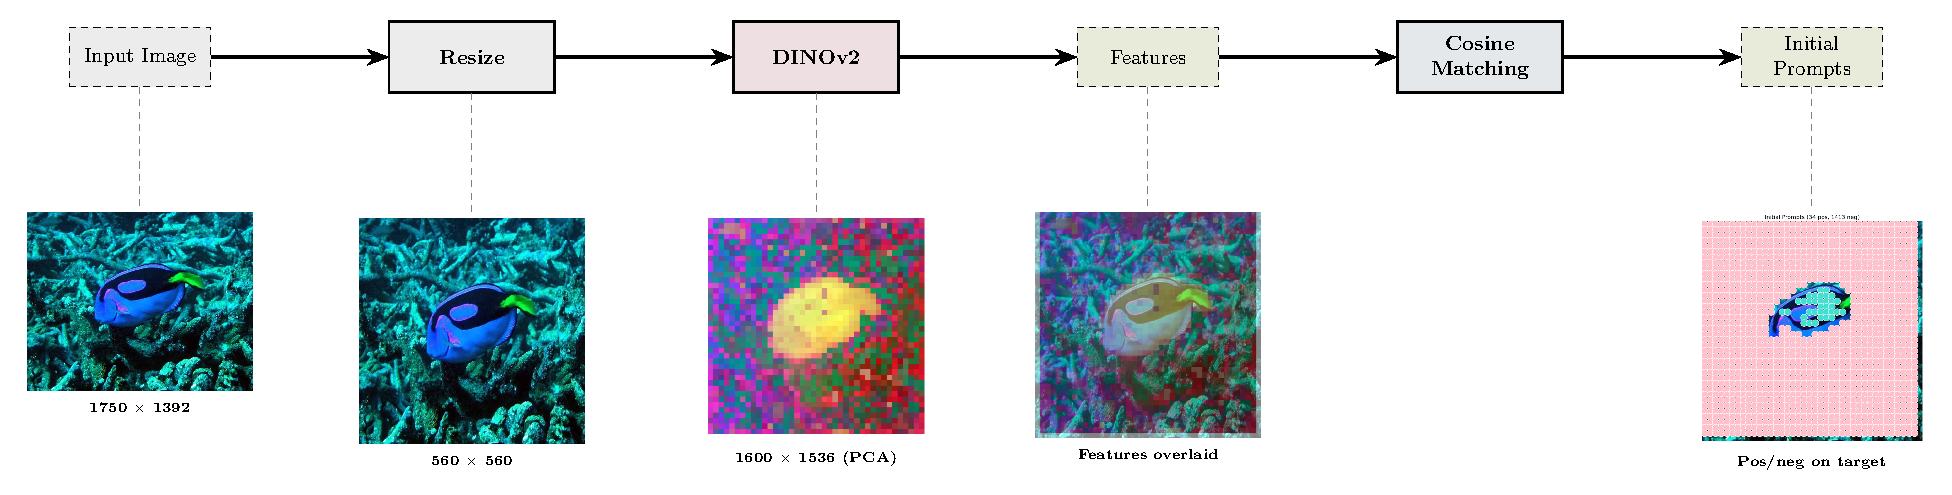
\includegraphics[width=\textwidth]{figures/fig_dino_detail.pdf}
\caption{DINOv2 feature extraction and cosine matching pipeline with real outputs.}
\label{fig:dino_detail}
\end{figure}

\subsection{Nearest-Neighbor Feature Matching}

For each foreground patch index $f_i \in \mathcal{F}$, the pipeline finds the target patch with the most similar DINOv2 feature vector using L2 distance.
\begin{align}
\texttt{pos}_i = \arg\min_{j \in \{1, \ldots, 1600\}} \left\| \mathbf{F}^{\text{ref}}_{f_i} - \mathbf{F}^{\text{tgt}}_j \right\|_2
\end{align}

This produces the \textbf{initial positive prompt indices} on the target image. The same process is applied to background patches $\mathcal{B}$ to get \textbf{initial negative prompt indices}. Any index appearing in both sets is removed from both to prevent contradictory prompts.

Figure~\ref{fig:step1} shows the Step 1 output. The left panel displays DINOv2 feature-matched prompts on the target image (34 positive, 1413 negative). The right panel shows the SAM mask produced with these unoptimized prompts. The initial IoU with ground truth is only 0.001 because feature matching produces many false positive and negative prompt locations.

\begin{figure}[H]
\centering
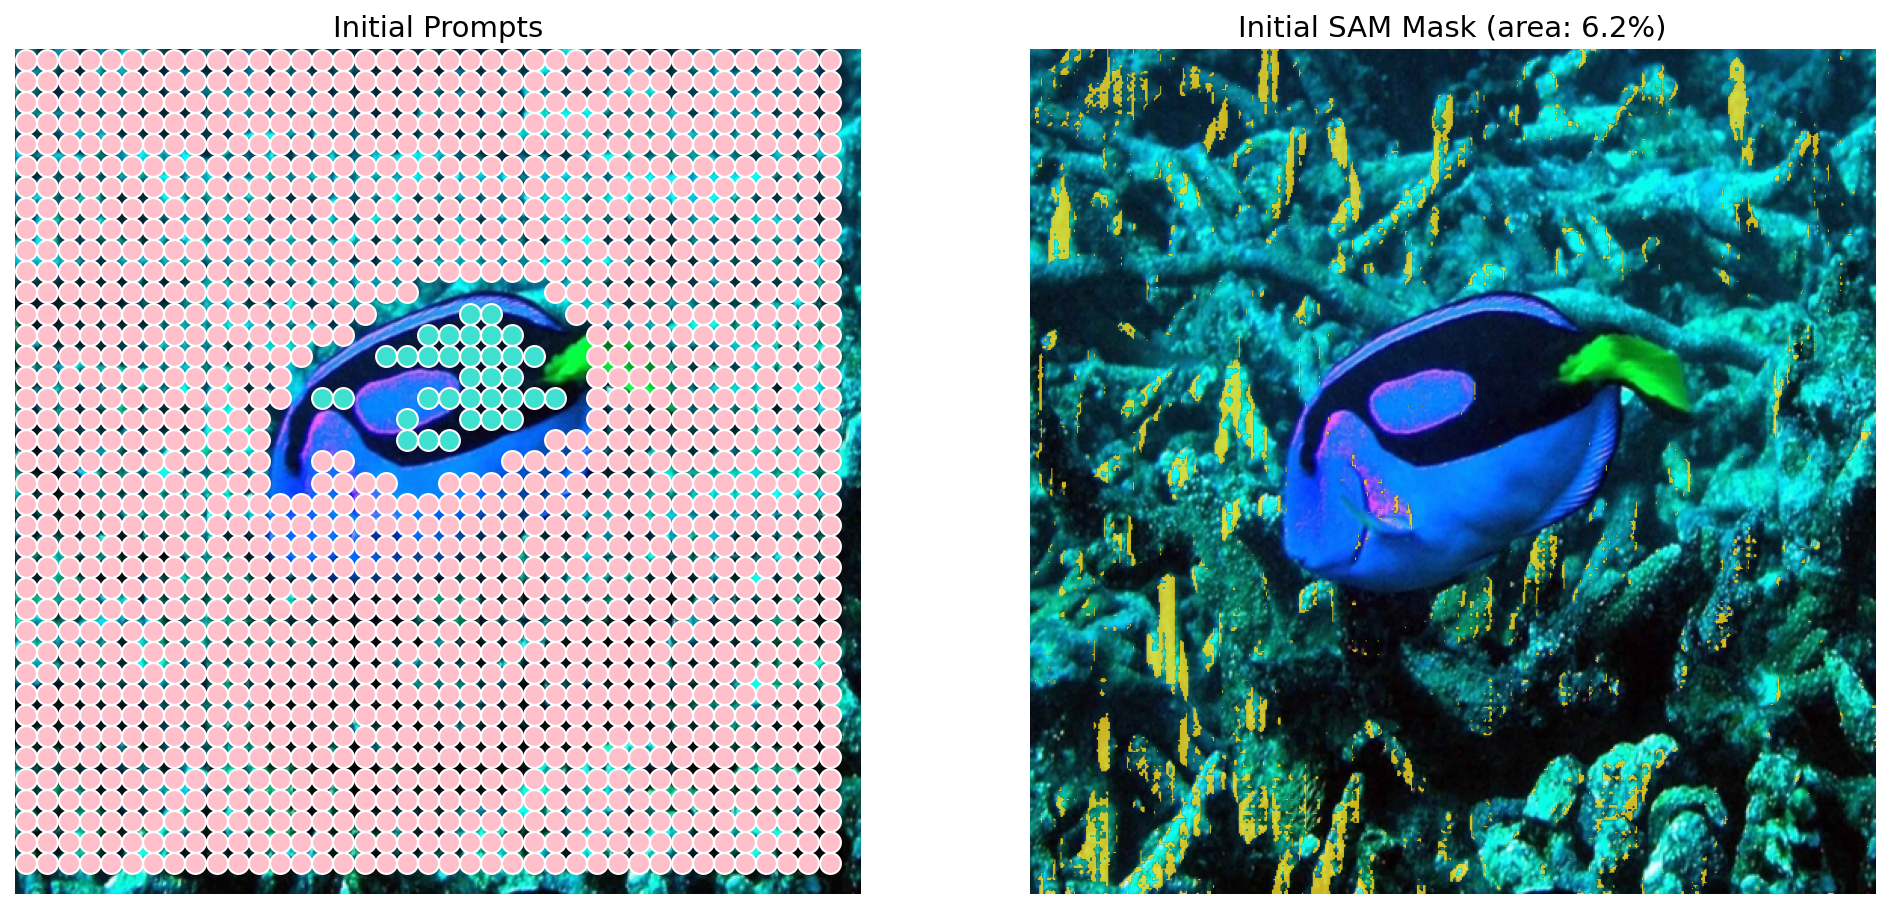
\includegraphics[width=0.85\textwidth]{figures/ppo_step1_initial_mask.png}
\caption{Step 1 output: initial prompts (left) and resulting SAM mask (right), IoU = 0.001.}
\label{fig:step1}
\end{figure}

\subsection{Step 1 Summary}

Step 1 outputs three artifacts used by Step 2.
\begin{itemize}[nosep]
\item \textbf{features}: DINOv2 patch features for both images, shape $[2, 1600, 1536]$
\item \textbf{pos\_indices}: Initial positive prompt patch indices on target (e.g., 34 patches for our blue tang)
\item \textbf{neg\_indices}: Initial negative prompt patch indices on target (e.g., 1413 patches)
\end{itemize}

These are the \textit{unoptimized} prompt candidates. SAM segmentation with these raw prompts typically produces poor results because nearest-neighbor feature matching gives many false positives and negatives.

% ============================================================
\section{Step 2: Q-Learning on Dual-Space Heterogeneous Graph}
\label{sec:step2}
% ============================================================

This is the core contribution of the paper. The pipeline constructs a graph encoding both semantic and spatial relationships between candidate prompts, then uses Q-learning to select the optimal subset.

\subsection{Graph Construction}

Each candidate prompt index becomes a \textbf{node} in a NetworkX MultiGraph, labeled as either \texttt{pos} (positive prompt) or \texttt{neg} (negative prompt). In our blue tang experiment, this produces $34 + 1413 = 1{,}447$ nodes.

The graph has \textbf{five distinct edge types}, each encoding pairwise distances between nodes in one of two spaces: DINOv2 feature space (semantic) or pixel coordinate space (physical). All distances are computed via L2 norm and then min-max normalized to $[0, 1]$.

Figure~\ref{fig:dsh_internals} illustrates the dual-space structure. The left panel shows DINOv2 feature space, where positive nodes (foreground prompts) and negative nodes (background prompts) are connected by feature-distance edges encoding semantic similarity. The right panel shows physical pixel space, where the same nodes are connected by spatial-distance edges encoding geometric arrangement. Five edge types span both spaces: \texttt{feature\_pos}, \texttt{feature\_cross}, \texttt{physical\_pos}, \texttt{physical\_neg}, and \texttt{physical\_cross}.

\begin{figure}[H]
\centering
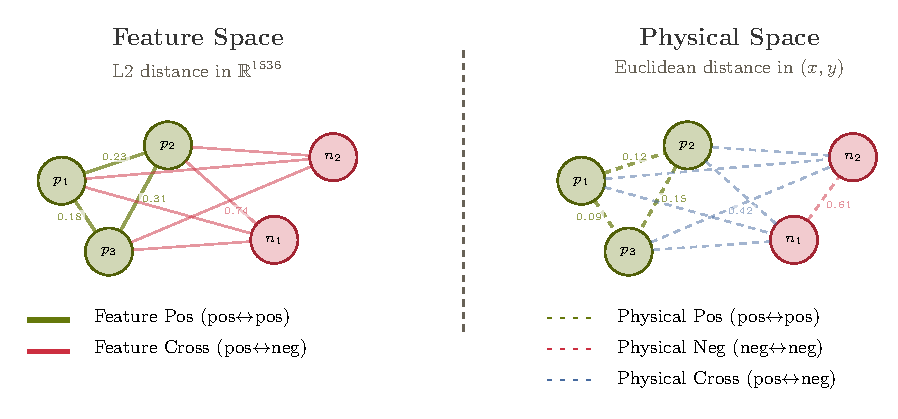
\includegraphics[width=\textwidth]{figures/fig_dsh_internals.pdf}
\caption{Dual-space heterogeneous graph: feature space (left) and physical space (right).}
\label{fig:dsh_internals}
\end{figure}

\begin{table}[H]
\centering
\caption{Five edge types in the dual-space graph.}
\label{tab:edges}
\begin{tabular*}{\textwidth}{@{\extracolsep{\fill}}lllp{5.5cm}@{}}
\toprule
\textbf{Edge Type} & \textbf{Space} & \textbf{Connects} & \textbf{Optimization Goal} \\
\midrule
\texttt{feature\_pos} & DINOv2 & pos $\leftrightarrow$ pos & Minimize (semantic cohesion) \\
\texttt{feature\_cross} & DINOv2 & pos $\leftrightarrow$ neg & Maximize (fg/bg separation) \\
\texttt{physical\_pos} & Pixel & pos $\leftrightarrow$ pos & Maximize (spatial spread) \\
\texttt{physical\_neg} & Pixel & neg $\leftrightarrow$ neg & Maximize (spatial spread) \\
\texttt{physical\_cross} & Pixel & pos $\leftrightarrow$ neg & Minimize (boundary proximity) \\
\bottomrule
\end{tabular*}
\end{table}

For our experiment with 34 positive and 1413 negative nodes, the fully-connected graph contains approximately \textbf{2,093,484 edges} across all five types. This is the primary computational bottleneck of the pipeline.

Figure~\ref{fig:graph_detail} traces this process with real pipeline outputs. Initial positive and negative prompt candidates from Step 1 are used to build the dual-space heterogeneous graph. The Q-learning agent then optimizes prompt selection over 30 episodes, reducing 1,447 candidates to 26 optimized prompts (6 positive, 20 negative) that produce a high-quality SAM segmentation mask.

\begin{figure}[H]
\centering
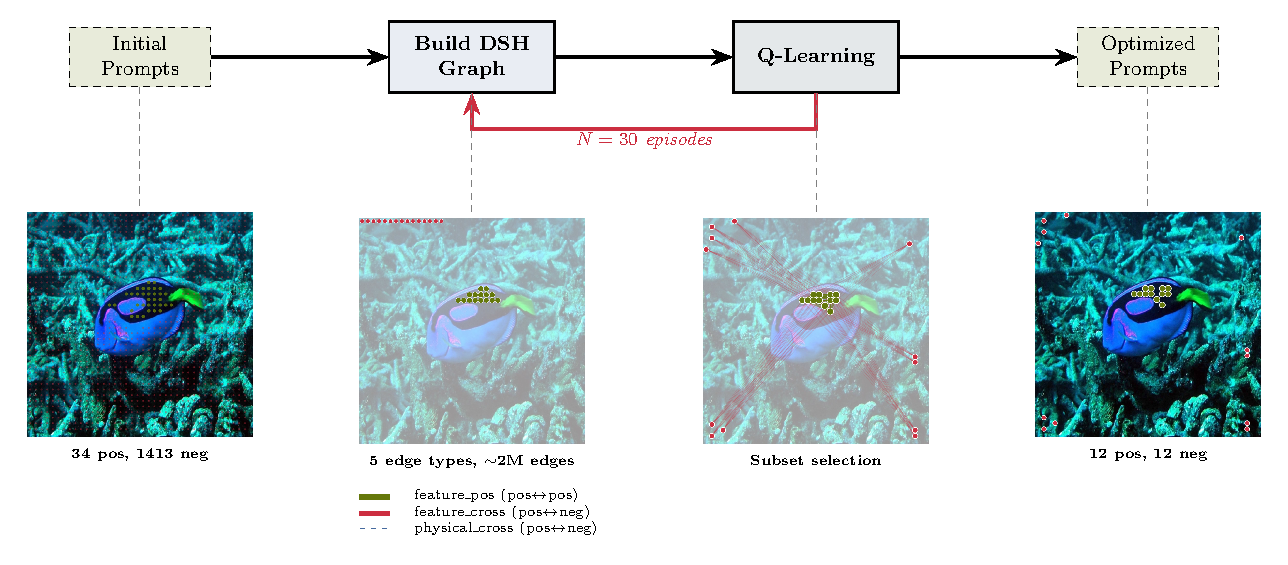
\includegraphics[width=\textwidth]{figures/fig_graph_detail.pdf}
\caption{Graph stage: from initial prompts through Q-learning optimization to final output.}
\label{fig:graph_detail}
\end{figure}

\subsection{Graph Optimization Environment}

The graph is wrapped in a reinforcement learning environment (\texttt{GraphOptimizationEnv}) with the following interface.

The state is the current graph $G = (V, E)$ with whatever nodes remain after agent actions, represented as a NetworkX MultiGraph object.

On each episode start, \textit{all nodes are removed} from the graph and placed in a ``removed'' set. The agent begins with an empty graph and must actively restore nodes. This makes the agent's task fundamentally one of \textit{subset selection}: choosing which of the 1,447 candidate nodes to include.

The agent can perform five types of actions at each step.

\begin{table}[H]
\centering
\caption{Action space. The agent manipulates individual nodes. Counts are constrained to $[5, 20]$ per category.}
\label{tab:actions}
\begin{tabular*}{\textwidth}{@{\extracolsep{\fill}}lp{9.5cm}@{}}
\toprule
\textbf{Action} & \textbf{Effect} \\
\midrule
\texttt{(node, restore\_pos)} & Restore a positive node from the removed set with all its original edges \\
\texttt{(node, restore\_neg)} & Restore a negative node from the removed set \\
\texttt{(node, remove\_pos)} & Remove a positive node currently in the graph \\
\texttt{(node, remove\_neg)} & Remove a negative node currently in the graph \\
\texttt{(node, add)} & Add a brand new node (randomly assigned pos/neg, penalized $-10$) \\
\bottomrule
\end{tabular*}
\end{table}

Each episode is fixed at $T = 100$ steps.

The environment enforces $5 \leq |\text{pos nodes}| \leq 20$ and $5 \leq |\text{neg nodes}| \leq 20$. If positive node count hits the minimum, only \texttt{restore\_pos} actions are available. If it hits the maximum, only \texttt{remove\_pos} is available. The same logic applies to negative nodes. Additionally, \texttt{remove\_pos} and \texttt{remove\_neg} action lists are subsampled to match lengths, ensuring balanced removal probability between the two categories.

\subsection{Reward Function}

The reward after each action is computed from the change in five mean edge-weight statistics. Let $\bar{d}^{(t)}_k$ denote the mean weight of edge type $k$ at step $t$, and let $\bar{d}^{(t-1)}_k$ denote the value before the action.

\begin{align}
r_t &= \underbrace{5 \cdot \text{sgn}^{-}(\Delta\bar{d}_{\texttt{feat\_pos}})}_{\text{feature cohesion}} + \underbrace{5 \cdot \text{sgn}^{+}(\Delta\bar{d}_{\texttt{feat\_cross}})}_{\text{feature separation}} + \underbrace{1 \cdot \text{sgn}^{+}(\Delta\bar{d}_{\texttt{phys\_pos}})}_{\text{pos spread}} \nonumber \\
&\quad + \underbrace{1 \cdot \text{sgn}^{+}(\Delta\bar{d}_{\texttt{phys\_neg}})}_{\text{neg spread}} + \underbrace{1 \cdot \text{sgn}^{-}(\Delta\bar{d}_{\texttt{phys\_cross}})}_{\text{boundary proximity}} - \underbrace{10 \cdot \mathbb{1}[\texttt{add}]}_{\text{add penalty}}
\end{align}

where $\text{sgn}^{-}(\Delta) = \bar{d}^{(t-1)} - \bar{d}^{(t)}$ (rewards \textit{decreases}; penalizes increases by the same magnitude) and $\text{sgn}^{+}(\Delta) = \bar{d}^{(t)} - \bar{d}^{(t-1)}$ (rewards \textit{increases}; penalizes decreases).

\begin{figure}[H]
\centering

\includegraphics[width=0.75\textwidth]{figures/fig_reward.pdf}
\caption{Composite reward function with five edge-statistic components.}
\label{fig:reward}
\end{figure}

Figure~\ref{fig:reward} summarizes the reward components. Five graph statistics are tracked after every action. Feature-space objectives (top two) are weighted $5\times$ more than physical-space ones (bottom three). An add-node action incurs a flat $-10$ penalty.

The intuition behind this reward design is that it encourages a prompt set where (1) positive prompts are semantically coherent --- they should all represent the target object in DINOv2 feature space, (2) positive and negative prompts are semantically distinct --- foreground vs.\ background should be easily distinguishable, (3) prompts are spatially well-distributed across the image for coverage, and (4) negative prompts lie near the object boundary to help SAM delineate edges. The feature-space objectives receive $5\times$ weight because semantic correctness is more important than spatial arrangement.

\subsection{Q-Learning Agent}

Despite the repository name ``PPO,'' the actual algorithm is \textbf{tabular Q-learning with experience replay}. There is no neural network policy, no clipping objective, and no advantage estimation. The name ``PPO'' refers to ``Plug-and-Play Optimization,'' not the RL algorithm.

The Q-table is a Python \texttt{defaultdict(float)} mapping $(s, a)$ pairs to scalar Q-values. The state key $s$ is the graph object reference; actions $a$ are tuples like $(\texttt{node\_id}, \texttt{"restore\_pos"})$.

The update rule follows standard Q-learning with learning rate $\alpha = 0.1$ and discount factor $\gamma = 0.9$:
\begin{align}
Q(s, a) \leftarrow Q(s, a) + \alpha \left[ r + \gamma \max_{a'} Q(s', a') - Q(s, a) \right]
\end{align}

Action selection follows an epsilon-greedy exploration schedule. Epsilon is reset at the start of each episode based on the best cumulative reward achieved so far.
\begin{align}
\epsilon_{\text{init}} = \begin{cases}
1.0 & \text{if } R_{\text{best}} < 0 \quad \text{(fully random)} \\
1 - R_{\text{best}} / 5 & \text{if } 0 \leq R_{\text{best}} < 5 \\
0.1 & \text{if } R_{\text{best}} \geq 5 \quad \text{(mostly greedy)}
\end{cases}
\end{align}
Within each episode, $\epsilon$ decays multiplicatively by $0.995$ after every step, so over 100 steps it decreases by roughly $\epsilon \times 0.995^{100} \approx 0.61\epsilon$.

Experience replay uses a ring buffer that stores up to 10,000 transitions $(s, a, r, s')$. After each step, a random mini-batch of 64 transitions is sampled and used for additional Q-table updates. When a new best episode reward is achieved, the current buffer is cloned as ``best memory'' and replayed to reinforce successful strategies.

\begin{table}[H]
\centering
\caption{Q-learning hyperparameters.}
\label{tab:hyperparams}
\begin{tabular}{@{}ll@{}}
\toprule
\textbf{Parameter} & \textbf{Value} \\
\midrule
Learning rate ($\alpha$) & 0.1 \\
Discount factor ($\gamma$) & 0.9 \\
Epsilon start & 1.0 \\
Epsilon end & 0.1 \\
Epsilon decay (per step) & 0.995 \\
Replay buffer size & 10,000 \\
Replay batch size & 64 \\
Steps per episode ($T$) & 100 \\
Min/Max nodes per category & 5 / 20 \\
\bottomrule
\end{tabular}
\end{table}

\subsection{Training Loop}

Each training episode proceeds as follows.

Figure~\ref{fig:qlearning_mdp} diagrams the MDP loop. The agent starts with an empty graph each episode and takes 100 actions (restore/remove positive or negative nodes) to build up a prompt set. At each step, the environment computes a reward from changes in mean edge weights across five graph statistics. The Q-table maps (state, action) pairs to values and is updated via standard Q-learning with experience replay. The best Q-table is saved when a new best cumulative reward is achieved.

\begin{figure}[H]
\centering
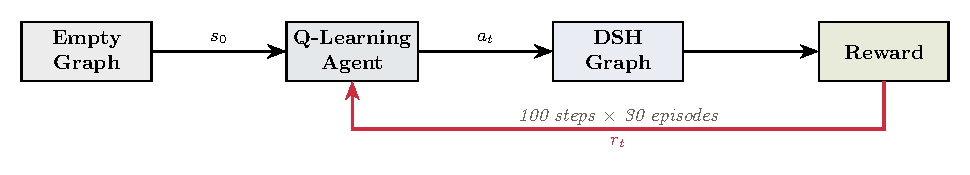
\includegraphics[width=0.85\textwidth]{figures/fig_qlearning.pdf}
\caption{Q-learning MDP loop for prompt subset selection.}
\label{fig:qlearning_mdp}
\end{figure}

Over training, the agent learns which specific patch indices to include. In our experiment, it consistently converges to approximately \textbf{6 positive and 20 negative nodes} from the original 1,447 candidates. The three ``best'' models are tracked independently: best by cumulative reward, best by feature cohesion (lowest mean \texttt{feature\_pos}), and best by feature separation (highest mean \texttt{feature\_cross}).

\subsection{Critical Design Decision: SAM is Not in the Training Loop}

SAM is \textbf{never called during Q-learning training}. The reward function is based entirely on graph statistics (mean edge weights). SAM is only invoked twice in the entire pipeline: once with initial prompts (to show the baseline) and once with optimized prompts (to produce the final mask). This makes training computationally feasible --- the reward is a \textit{proxy} for segmentation quality rather than a direct measure of it. The proxy works because the five graph objectives (feature cohesion, feature separation, spatial spread, and boundary proximity) correlate well with SAM's ability to produce accurate masks from the resulting prompt set.

% ============================================================
\section{Step 3: SAM Segmentation with Optimized Prompts}
% ============================================================

\subsection{Prompt Optimization at Inference}

Using the trained Q-table, the agent runs one final episode with reduced exploration ($\epsilon \approx 0.1$). Starting from an empty graph, it restores and removes nodes over 100 steps. The surviving nodes become the optimized prompt set.

Each patch index is converted to pixel coordinates.
\begin{align}
(x, y) = \left( (i \bmod 40) \times 14 + 7, \; \lfloor i / 40 \rfloor \times 14 + 7 \right)
\end{align}

\subsection{SAM Prediction}

The optimized coordinates are passed to \textbf{SAM ViT-B} (358 MB checkpoint) as point prompts.
\begin{align}
\texttt{mask} = \text{SAM}\!\left(I_{\text{tgt}}, \; \{(x_i, y_i, \ell_i)\}_{i=1}^{N_{\text{pos}} + N_{\text{neg}}}\right)
\end{align}
where $\ell_i = 1$ for positive prompts and $\ell_i = 0$ for negative. SAM's \texttt{multimask\_output} is set to \texttt{False}, producing a single best mask.

\newpage

% ============================================================
\section{Limitations for Few-Class Detection}
\label{sec:limitations}
% ============================================================

The PPO pipeline was designed for general one-shot segmentation, where the target class is unknown at design time and only a single reference example is available. However, many practical deployment scenarios involve detecting a small number of known classes repeatedly --- for example, identifying one or two fish species across thousands of underwater video frames. In this regime, the pipeline exhibits several fundamental limitations that make it poorly suited compared to conventional approaches.

\subsection{No Generalization Across Images}

The entire pipeline --- DINOv2 feature extraction, graph construction, and Q-learning optimization --- runs from scratch for every new target image. The Q-table maps specific patch indices to Q-values, meaning it is entirely image-specific with zero transfer to any other image. For a production system detecting 1--2 classes in a video stream, this means spending $\sim$50 minutes per frame. Even at reduced episode counts, the per-image computational overhead is dominated by the $O(n^2)$ graph construction and the iterative Q-learning loop, neither of which amortize across images. A system that requires complete retraining for every input is fundamentally incompatible with real-time or batch processing requirements.

\subsection{DINOv2 ViT-G/14 is Massive Overkill}

DINOv2 ViT-G/14 was designed for general-purpose visual understanding across thousands of semantic categories. Its 1.1 billion parameters and 1536-dimensional patch features encode a vast representational capacity that is entirely unnecessary for distinguishing 1--2 known classes from their typical backgrounds. For narrow-scope detection tasks, a fine-tuned lightweight backbone such as ResNet-50 ($\sim$25M parameters), MobileNetV3 ($\sim$5M parameters), or even DINOv2 ViT-S/14 ($\sim$22M parameters) would produce sufficient feature discrimination at a fraction of the computational cost. The 4.2 GB checkpoint download and $\sim$16 GB VRAM requirement are wasteful when the feature space needs to separate only two clusters instead of thousands.

\subsection{The $O(n^2)$ Graph is Computationally Absurd for Few Classes}

The dual-space heterogeneous graph is fully connected within and across node categories, producing $O(n^2)$ edges where $n = N_{\text{pos}} + N_{\text{neg}}$. With 1,447 nodes in our experiment, this yields approximately 2 million edges, each of which must be recomputed or queried at every Q-learning step. For 1--2 known classes, the feature distributions are well-characterized from training data. A simple threshold on cosine similarity (e.g., ``include patches with $\text{sim}(f_i, \mu_{\text{class}}) > \tau$'') would achieve the same semantic filtering that the graph-based optimization labors to discover. The graph representation adds $O(n^2)$ complexity to solve a problem that has an $O(n)$ solution when class prototypes are known.

\subsection{Proxy Reward Never Optimizes Actual Segmentation Quality}

The Q-learning reward is computed from changes in mean edge weights --- feature cohesion, feature separation, spatial spread, and boundary proximity. SAM is called only once at the very end of the pipeline, meaning the agent never receives feedback about the actual segmentation quality it produces. The reward is a proxy, and proxies can diverge from the true objective. In our experiment, the best Q-learning reward did not correspond to the best IoU: the checkpoint run achieved its highest IoU (0.638) at episode 5, while the reward continued to improve through later episodes that produced worse masks. For few-class detection where ground truth is abundant from training data, directly optimizing IoU via gradient-based methods (e.g., differentiable prompt optimization or end-to-end fine-tuning) would be far more effective than relying on a proxy that is only loosely correlated with mask quality.

\subsection{Tabular Q-Learning Does Not Scale}

The Q-table is keyed on (graph object reference, action tuple) pairs with no function approximation. This means the agent cannot generalize from one graph configuration to a similar one --- every state is treated as entirely novel. With 1,447 nodes and 5 action types, the effective action space is $\sim$7,200 discrete options, but the agent takes only 3,000 total steps across 30 episodes (100 steps each). The Q-table is therefore extremely sparse, with most state-action pairs never visited. This sparsity explains the high variance in training dynamics visible in the IoU progression: the agent has not explored enough of the space to converge reliably. A function approximator (e.g., a small neural network mapping graph statistics to action values) would generalize across similar states, but this would transform the algorithm into something fundamentally different from the tabular approach presented.

\subsection{The One-Shot Premise is Unnecessary for Known Classes}

The entire pipeline is engineered around the constraint that only a single reference example is available. This is a genuinely challenging and useful setting for novel object discovery. However, if the deployment task always involves the same 1--2 classes, this constraint is artificial. With many available training examples, a fine-tuned segmentation model --- Mask R-CNN, YOLO-Seg, or a fine-tuned SAM with learned prompt embeddings --- would outperform this pipeline while requiring only a single forward pass at inference time (milliseconds, not minutes). The one-shot formulation introduces unnecessary complexity when the few-class assumption guarantees abundant supervision.

\subsection{Single Forward Pass SAM Bottleneck}

SAM is called once with all optimized prompts simultaneously, producing a single mask with no opportunity for refinement. If the prompt set contains even one misplaced point, the mask quality degrades with no recovery mechanism. For known classes, an iterative approach --- predict a mask, evaluate it against class priors, refine prompts based on the intermediate result, and re-predict --- would be substantially more robust. The current pipeline's rigid separation between prompt optimization (graph domain, no SAM feedback) and mask generation (single SAM call, no prompt correction) leaves significant performance on the table.

\end{document}
